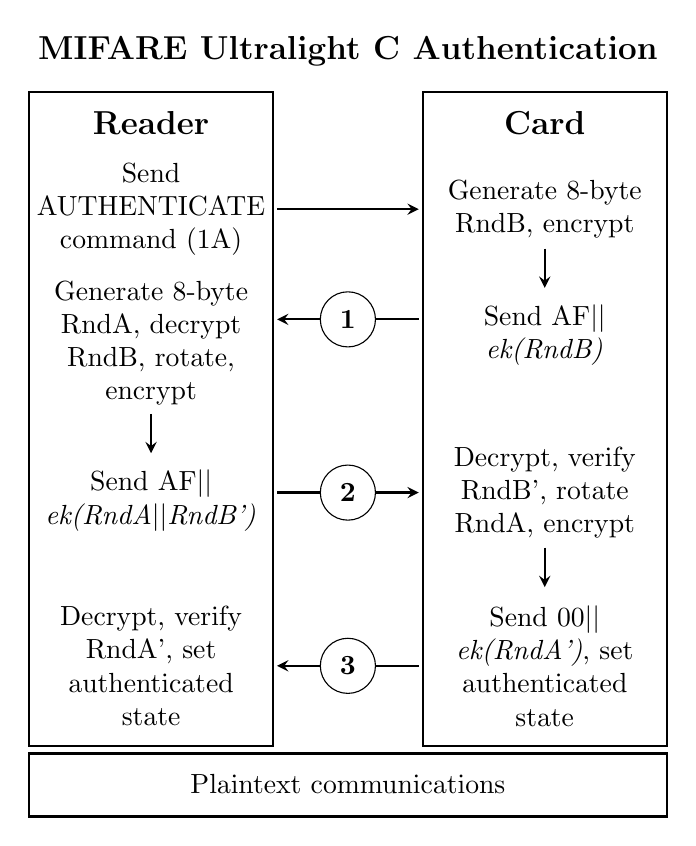
\begin{tikzpicture}[
    % Define styles
    box/.style={
        rectangle, 
        draw, 
        thick,
        minimum width=3.1cm, 
        minimum height=8.3cm,
        anchor=north
    },
    plaintext/.style={
        rectangle, 
        draw,
        thick,
        minimum width=8.1cm, 
        minimum height=0.8cm,
        anchor=north
    },
    arrow/.style={
        ->, 
        >=stealth,
        thick
    },
    numbered/.style={
        circle,
        draw,
        fill=white,
        minimum size=0.7cm,
        font=\bfseries
    }
]

% Set up the coordinate system
\def\yshift{0}

% Title
\node[font=\large\bfseries] at (-2.5,\yshift+4.0) {MIFARE Ultralight~C Authentication};
%\node[font=\large] at (-2.5,\yshift+4.0) {3-Pass Mutual Authentication};

% Draw reader box
\node[box, fill=none, anchor=north] (reader) at (-5,\yshift+3.5) {};
\node[font=\large\bfseries] at (-5,\yshift+3.1) {Reader};

% Draw card box
\node[box, fill=none, anchor=north] (card) at (0,\yshift+3.5) {};
\node[font=\large\bfseries] at (0,\yshift+3.1) {Card};

% Draw box for plaintext communication
\node[plaintext, fill=none, anchor=north] (card) at (-2.5,\yshift-4.9) {};

% Reader side texts
\node[align=center] at (-5,\yshift+2.0) {Send\\AUTHENTICATE\\command (1A)};
\node[align=center] at (-5,\yshift+0.3) {Generate 8-byte\\RndA, decrypt\\RndB, rotate,\\encrypt};
\node[align=center] at (-5,\yshift-1.7) {Send AF\textbar\textbar\\\textit{ek{(}RndA{\textbar}{\textbar}RndB'{)}}};
\node[align=center] at (-5,\yshift-3.8) {Decrypt, verify\\RndA', set\\authenticated\\state};

% Card side texts
\node[align=center] at (0,\yshift+2.0) {Generate 8-byte\\RndB, encrypt};
\node[align=center] at (0,\yshift+0.4) {Send AF\textbar\textbar\\\textit{ek{(}RndB{)}}};
\node[align=center] at (0,\yshift-1.6) {Decrypt, verify\\RndB', rotate\\RndA, encrypt};
\node[align=center] at (0,\yshift-3.8) {Send 00\textbar\textbar\\\textit{ek{(}RndA'{)}}, set\\authenticated\\state};

% Internal arrows in reader
\draw[arrow] (-5,\yshift-0.6) -- (-5,\yshift-1.1);
%\draw[arrow] (-4,\yshift-2) -- (-4,\yshift-3.8);

% Internal arrows in card
\draw[arrow] (0,\yshift+1.5) -- (0,\yshift+1.0);
\draw[arrow] (0,\yshift-2.3) -- (0,\yshift-2.8);

% Communication arrows between boxes
% Top arrow - Send Authenticate command
\draw[arrow] (-6+2.6,\yshift+2) -- (1-2.6,\yshift+2) node[midway, above, font=\small] {};
%\node[circle, draw, fill=white, minimum size=0.7cm, font=\bfseries] at (-2.5,\yshift+2) {1};

% First pass
\draw[arrow] (1-2.6,\yshift+0.6) -- (-6+2.6,\yshift+0.6) node[midway, below, font=\small] {};
\node[circle, draw, fill=white, minimum size=0.7cm, font=\bfseries] at (-2.5,\yshift+0.6) {1}; % 2

% Second pass
\draw[arrow] (-6+2.6,\yshift-1.6) -- (1-2.6,\yshift-1.6) node[midway, below, font=\small] {};
\node[circle, draw, fill=white, minimum size=0.7cm, font=\bfseries] at (-2.5,\yshift-1.6) {2}; % 3

% Third pass (top of the numbered ones)
\draw[arrow] (1-2.6,\yshift-3.8) -- (-6+2.6,\yshift-3.8) node[midway, below, font=\small] {};
\node[circle, draw, fill=white, minimum size=0.7cm, font=\bfseries] at (-2.5,\yshift-3.8) {3}; % 4

\node[align=center] at (-2.5,\yshift-5.3) {Plaintext communications};
\end{tikzpicture}
